\chapter{架构设计}
\label{chap:system-framework}
当系统需求和输入输出明确以后,首先要做的就是系统的架构设计。一个好的架构设计能让系统层次简明,易于理解,各构件各司其职,从而有效提高系统的效率、稳定性、安全性、扩展性和可维护性。

\section{框架设计}
从之前的需求分析来看,病人病历自动生成与归档系统从输入图片数据,到最终输出的文档数据,需经过若干个数据加工处理步骤,这些步骤之间是顺序依次执行的,并且模块之间没有相互的反馈关系,即模块间以线性展开,没有环路,这天然构成了系统架构设计中的管道模式(Pipeline Pattern)\citep{Vermeulen1995pipeline},或称过滤器模式(Filter Pattern)。管道/过滤器模式的软件架构,是系统架构中的一种非常常见的形式,系统中每个模块都有输入输出,数据以流的形式向下传递。
它具有结构简明、扩展性好、易于维护、支持并行执行等很多优点。
具体到本系统来说,基于管道式的架构设计思想,我们可以将整个系统分成若干个处理模块,一组数据流将这些处理模块串联起来,数据流以每个病人的病历数据为单位,从输入口经过一系列加工处理,得到最终的输出,各个病人病历之间互不干扰,犹如生产线一般严格产出。

确定了采用管道式的系统架构后,接下来我们可以结合问题需求,按照数据流的顺序,一步步设计管道中的构件(模块)。首先,我们需将输入的图片数据作为数据流的开端,让我们乘着数据的一叶扁舟,顺流而下,逐一分析与设计。

\section{模块设计}
\subsection{数据加载模块} \label{ssec:dataLoader-design}
数据加载模块是数据流的入口,病人病历数据以多张图片的形式输入,对于计算机而言,是无法判断某张图片是属于哪个病人的,如果不对这些图片数据进行标识,很容易出现张冠李戴的现象,现实中如果将病人A的诊疗数据误录入到病人B的病历档案中,一方面病人A的诊疗数据就此丢失,医生做诊断的时候就没法做到全面,另一方面,更严重的是医生对病人B的诊断依据的是完全错的历史诊疗记录,很可能对病人B做出不恰当的诊断,这种误诊造成的伤害是不可估量的。因此,系统对输入数据应提出这样的需求,即每个病人的病历数据应该具有唯一的标识,如图片名字拥有唯一的前缀等。而数据加载模块,就可以根据这样的标识,来给海量的图片数据做好分门别类的工作,确保数据以病人为原子单位向后传递。

\subsection{版面分析模块} \label{ssec:framework-segmentation-analysis}
当数据到达版面分析模块时,数据流中流淌的仍然是图片数据。这些图片数据中的每个“原子数据“是以病人为单位构成的一组图片集合,假设每个病人的病历数据对应着10张图片,这些图片间的病历信息互不重叠,是病历数据的有序记录,那么一个现实的问题是,当一组图片数据到来时,系统如何判断它们之间的次序,或者说某张图片中期望获得的字段数据有哪些呢?这就要求版面分析具有的第一个功能就是分辨这一组10张图片的总体属性,如果说数据加载模块是将图片数据以病人为单位做了第一步的划分,那么版面分析模块就是在此之上以图片为单位做的第二层划分。

版面分析模块的使命不止于此,当划分好每张图片后,图片中仍然存有着大量的冗余干扰信息,如\autoref{pic:input-image-1}中所示,图中除了需要识别的主题内容外,还存在着系统信息、侧边栏列表等无关信息,版面分析模块需要剔除这些干扰信息,分离出病历主题内容。

最后,对于提取出的病历主体内容,其实仍然存在着大片的空白,如果直接将它传递给下游的文字识别模块,文字相对于图片过于稀疏,识别准确率肯定大打折扣,而且识别出来的文字包含有多个字段,要从这些文字中正确解析各个字段,难度也不小。因此,版面分析模块还需要从主体内容中剔除空白内容,将各个字段提取出来,形成若干个子图片,这些子图片只包含文字区域,一个子图片对应一个字段,这样,既能有效提高后续文字识别模块的准确率,又能降低字段解析的难度,可谓一举两得。

从上面的分析来看,版面分析模块应该具备以下功能:
\begin{itemize}
	\item 对病历图片进行二次分类;
	\item 剔除图片中的干扰信息,获得病历数据主体;
	\item 剔除主体内容中的空白,提取出各个字段。
\end{itemize}
不难发现,版面分析模块本身,也可以认为是一个管道模式架构设计。

\subsection{预处理模块}
提取出来的字段图片,虽然以文字为主体,但是文字本身很可能是比较小的,从\autoref{pic:input-image-1}中就不难看出,这样的文字大小对人来说尚且有一定的辨识难度,遑论机器了,如果直接将这些图片数据传入文字识别系统进行识别,准确性可想而知。因此,我们需要对这些文字进行必要的预处理工作,在不改变文字本身线条和结构特性的前提下,尽量放大文字尺寸和它的轮廓特征,以便文字识别模块的识别,在光学字符识别领域,预处理的好坏往往能大大影响识别精度,好的预处理能让文字识别事半功倍,反之则会成为识别精度提升的瓶颈。

\subsection{OCR模块}
接下来自然来到了整个文字识别的核心:光学字符识别(OCR)模块。光学字符识别在印刷体识别领域的应用由来已久\citep{impedovo1991optical},技术也早已成熟,其本质是一个分类器,只是输入数据被限制为图片,输出数据为文本。当识别场景简单明确时,现有的OCR技术的识别精度已经高,但是当识别场景复杂,杂讯干扰较多时,识别效果会大打折扣。所以,如果要优化OCR模块的识别效果,一方面可以从优化分类器入手,如有针对性的设计数据集、增大训练样本数量等。另一方面,就是通过前置预处理模块,将识别问题简化,有关OCR的优化,在第四章中会有更加详细的论述。
数据流经过这一个模块之后,从图片转换成了文本。

\subsection{字段解析模块}
经过OCR模块的处理,图片转换成了文字,是不是意味着大功告成了呢?显然不是。首先一个问题,就是系统其实并不能从语义上理解识别出来的文字的,因此对于机器来说,这无非是从一种无法理解的数据转换成了另外一种无法理解的数据;其次,经过OCR模块识别出来的文本,带有某些冗余信息或者是错误信息,需要进行进一步的文本清洗和矫正工作。因此,我们需要加入一个字段解析模块,既负责文本的清洗矫正工作,又承担字段解析的功能。这个模块也可以成为“后处理模块”,是对识别文本的进一步优化。

\subsection{数据存储模块}
字段被解析出来后,应该如何存储呢?这就需要我们整个系统最后一个模块的引入:数据存储模块。在\autoref{chap:requirements-analysis}中我们提到,需求方期望的输出是有一定的数据组织形式和一定可读性的最终数据,数据存储模块就是承担着数据格式的组织和存储工作的,输入数据流经过它的转化之后,得到最终的需求输出。
\begin{figure}[htbp]
	\centering
	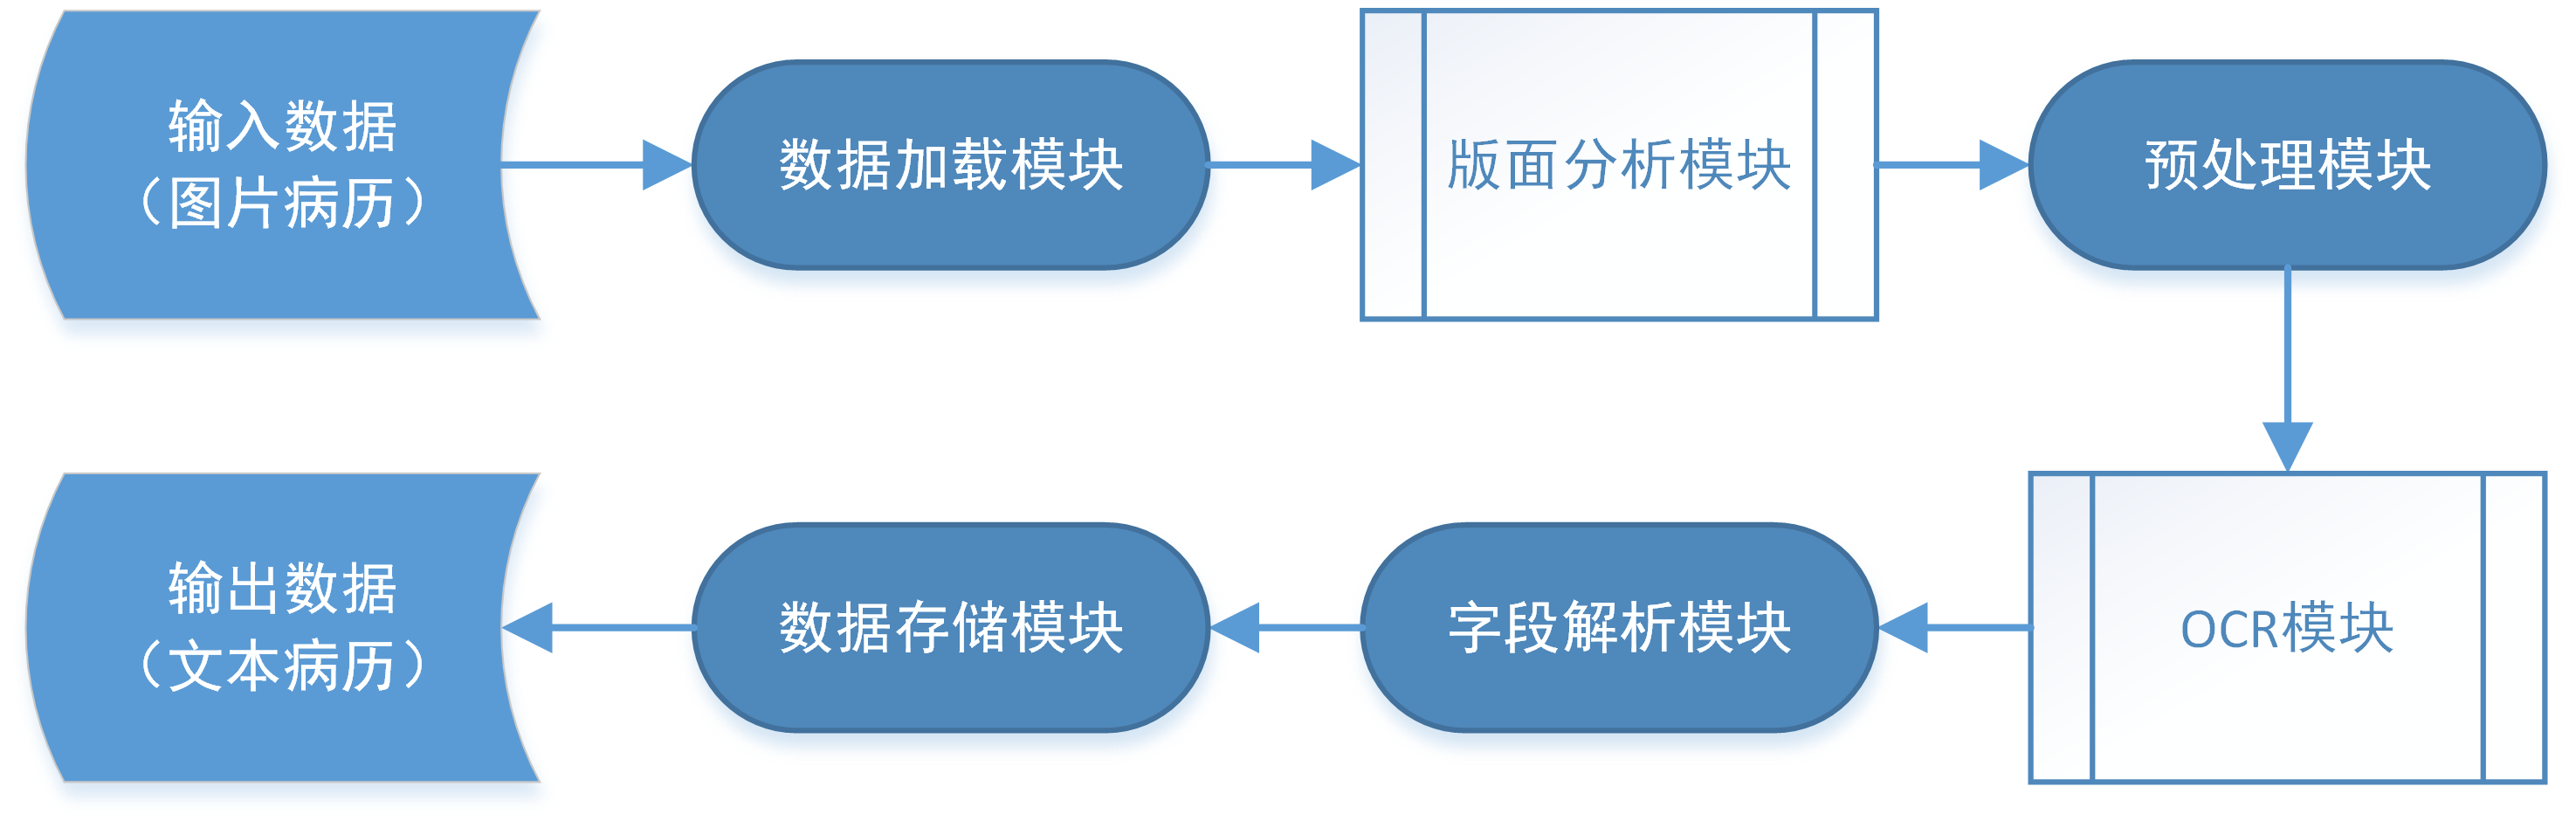
\includegraphics[width=0.9\textwidth]{system-framework}
	\caption{系统的整体架构设计}
	\label{pic:system-framework}
\end{figure}

\section{小结}
至此,我们根据病人病历自动生成与分类问题的实际需求,完成了一个管道模式/过滤器模式(Pipeline Pattern/ Filter Pattern)的系统框架设计,系统整体框架如\autoref{pic:system-framework}
所示,包含六个模块,模块间由数据流贯穿连接。这个框架即有一定的理论支撑,又结合了病历系统的实际,具备比较高的可行性。
